%!TEX root = report.tex

\section{Methods}\label{sec:methods}

\subsection{Environment}\label{sec:environment}
\begin{figure}[h]
    \centering
    \includegraphics[width=\linewidth]{img/simulation.png}
    \caption{Visual representation of the cellular automaton.}
    \label{fig:simulation}
\end{figure}
The forest fire is simulated using a cellular automaton. For a visual representation please see Figure \ref{fig:simulation}. Its shape is always square and has either a size of 10 or 14 cells. The green cells represent trees and can ignite under the right circumstances.
The agent (or bulldozer) is represented by the white tile. Wherever it moves it destroys the trees and an empty, inflammable (brown) cell is formed. A line of these dug cells forms a fire line over which the fire cannot spread. The agent has to move each time step, as it is not allowed to idle on the same cell. The agent can only die when it moves into an actively burning (red) cell.

\subsubsection{Fire Spread Dynamics}\label{sec:fire_spread}
When a tree is lit on fire in order to start a forest fire, the cell color switches from green to red in Figure \ref{fig:simulation}. The neighbouring cells start to heat up and switch to yellow. The term neighbouring cells refers to the cells directly north, south, east and west of a burning cell. After some time steps these neighbours reach their ignition thresholds they catch fire themselves. The larger the fire, the more cells are being heated and brought to ignition. This makes larger fires harder to contain. Each tile has a fixed amount of fuel and when it runs out of fuel, the fire dies out. This leaves behind a black burnt tile which cannot be reignited.


\subsubsection{The Reward function}\label{sec:reward_function}
The reward function is a function that maps each state to a value that represents how "good" or desirable that state is. As such, this function is a vital part of the learning process because any reinforcement learning algorithm will rely on the two things that constitute the input to the agent. The quality of the state representation, or in other words how much of- and how well the agent sees the environment, and the quality of the reward function, or how well the agents notion of success corresponds with our notion of success and how easy it is to find optima in the reward landscape.

Apart from determining the optimal policy to be learned by the agent, the reward function also determines the speed at which the agent will be able to learn that policy. To take the gradient descent analogy of a problem landscape, if the reward function produces a smooth gradient to the optimal solution, the agent will be able to find a path to that solution more easily than if the reward resembles flat landscape with sparse spikes in which the value jumps from almost always 0 or negative to a positive reward. In other words, the agent should be provided gradual feedback instead of sparse and delayed rewards in order to facilitate fast and efficient learning.

% provide references for reward claims

Crafting a good reward function for this problem turned out to be quite difficult because it was hard to define a measure of success that is both valid in its formulation and which provides gradual feedback, or a smooth gradient, towards the containment of the fire. We defined the reward function as
\[
R = \left\{\begin{array}{lr}
    1000, & \text{ Fire is contained }\\
    1000 * (p), & \text{ Fire burns out }\\
    -1000, & \text{ Agent dies }\\
    -1 & \text{ Otherwise }

    \end{array}\right\}
\]
where~$p$ is the percent of the map undamaged by either fire or digging. We decided to choose a reward function that defines the goal well, and then compensate for the lack of a smooth gradient with demonstration data to lead it towards the sparse rewards. Note that the 2nd and 3rd states are the only terminal states.

Containment of the fire is defined in \ref{alg:containment}. The algorithm returns true as soon as it can find a path, not allowing diagonal movements, between any burning cell and any cell on the border of the map. If there exists a path, then there exists a way for the fire to spread. It uses the A* path-finding algorithm to check for a path between any two points.

\begin{algorithm}
  \caption{Algorithm to check if the fire is contained}
  \label{alg:containment}
  \begin{algorithmic}[1]
    \Procedure{fireIsContained}{}
    \State {F = set of burning cells}
    \State {f = pop(F)}
    \State {B = set of burning cells}
    \State {b = pop(B)}
    \State {p = astarpath(f, b)}
    \While {p is not a path}
    \If {B is empty}
    \If {F is empty}
    \State \Return {True}
    \Else
    \State {B = set of border cells}
    \State {f = pop(F)}
    \EndIf
    \Else
    \State {b = pop(B)}
    \State {p = astarpath(f, b)}
    \EndIf
    \EndWhile
    \State \Return {False}
    \EndProcedure
  \end{algorithmic}
\end{algorithm}



\subsubsection{The State Representation}\label{sec:state_rep}
The state of the environment, or the observation of the environment as it is visible to the agent, consists of 3 matrices of size $N*M$ with a boolean domain resulting in, after flattening, an array of $3 * N*M$ boolean inputs where $(N, M)$ are the dimensions of the map. Assuming the shape of the map is always square, a map size of $N=10$ elements is represented three times: One layer contains only the agent position, translating to a matrix of zeros except for a single one representing the position of the agent. The second layer consists of the position of the fire. Cells that are on fire are represented by a 1, the rest are set to 0. The third layer represents the fire lines cut by the agent in a similar boolean fashion, resulting in a total of 300 inputs to the agent. This is schematically shown in figure \ref{fig:visiongrid}.

\begin{figure}[h]
    \centering
    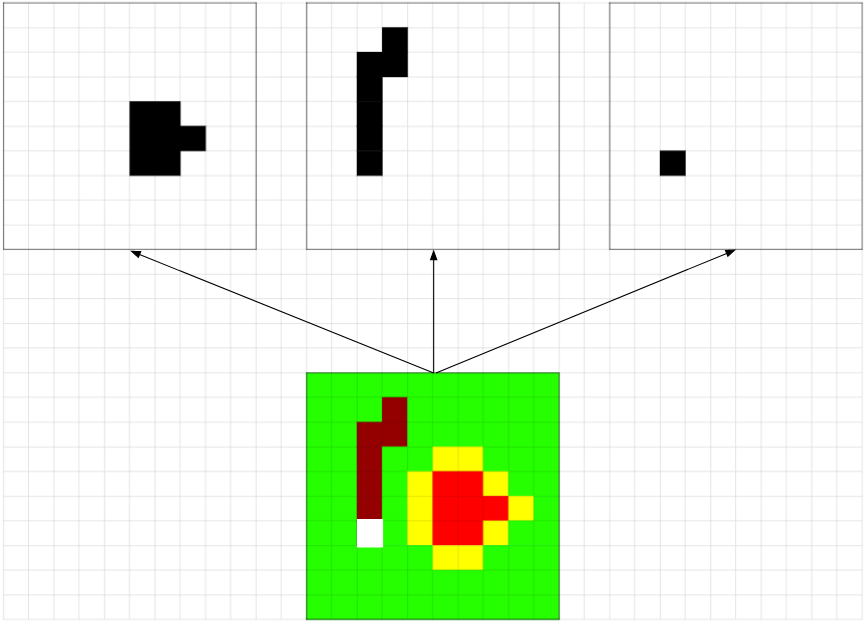
\includegraphics[width=1\linewidth]{img/Vision_Grid.png}
    \caption{A vision grid representation of an example state}
    \label{fig:visiongrid}
\end{figure}

This vision grid approach can speed up the learning process as well as increase the performance \citep{knegt2018opponent}. Indeed it had a noticeable effect on the performance and learning speed of our implementation compared to a single matrix representing the gray-scaled map as input, likely because the agent can more easily differentiate between different attributes and because only the relevant information is presented. Further, the agent can now see whether the cell it is occupying is already dug or not.


\subsection{The Agent}\label{sec:agent}


\subsubsection{Known Problems with Connectionist RL}\label{sec:problems}
The combination of function approximation (the neural network), bootstrapping (TD methods that update Q-values using estimated return values) and off-policy training (the Q-Learning algorithm) make up the deadly triad \citep{sutton_barto_2018}, which is known to cause instabilities and even divergence in the learning process. There are two well known strategies to reduce this effect and stabilise learning, using experience replay and a target network \citep{mnih2015human}.

\subsubsection{Experience Replay}\label{sec:exp_replay}

\begin{figure}[h]
    \centering
    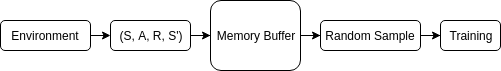
\includegraphics[width=1\linewidth]{img/Experience_Replay.png}
    \caption{Schematic structure of experience replay}
    \label{fig:expreplay}
\end{figure}

Instead of training the network on incoming experiences directly, the experiences can be stored in a memory buffer and the network can be trained on a mini-batch of memories randomly sampled from this buffer (see figure \ref{fig:expreplay}). This helps because neural networks assume that each training sample is identically and independently distributed with regard to the population the algorithm is set up to approximate (Citation needed), and training directly on incoming experiences break this assumption in two regards.

For one, consecutive incoming experiences are obviously highly correlated because the environment does not radically change after any action (unless it leads to a terminal state). This means that any experience differs from the previous experience only to the extent to which the environment can change in one update step from a single action from the agent. (Citation needed)

The distribution of incoming experiences is also dependent on the agents current policy. If the current policy determines that the agent should head east, then the next experiences recorded by the agent will involve the agent headed east. Apart from the obvious correlation, this can also lead to feedback loops (Explain the loops and cite dqn + paper below)

% https://arxiv.org/pdf/1511.05952.pdf
%(Check out the link for good reasons why experience replay is useful. already in .bib file)

% fill out the rest of the references

In addition to stabilising the learning process, this approach also increases sample efficiency by allowing memories to be re-used multiple times until they are discarded when they reach the end of the queue. We can also inject hand-crafted memories into this buffer before learning to provide the agent with demonstration, as will be explained in \ref{sec:demo_data}.


\subsubsection{Target Network}\label{sec:target_network}
Another source of instability is that we use the predictions of the network to generate the target values which, combined with the rest of the update rule (shown in figure \ref{fig:ql_sarsa}), directly update the weights of that same network. This can lead to unwanted feedback loops. We can add a delay to the loop to reduce these effects by using a periodically updated, frozen copy of the network to generate the target values instead (as shown in \ref{fig:targetnet}). Every C iterations, the target network is replaced by a copy of the main network. This modification is called Double Q-Learning \citep{NIPS2010_3964}, and was also used by \citep{mnih2015human} to make the algorithm more stable and prevent divergence.

\begin{figure}[h]
    \centering
    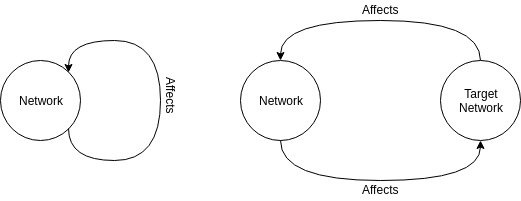
\includegraphics[width=1\linewidth]{img/Target_Network.png}
    \caption{Highlighting the schematic difference of using a target network}
    \label{fig:targetnet}
\end{figure}


\subsubsection{Q-Learning vs SARSA}\label{sec:ql_sarsa}
We implemented both Q-learning and SARSA to investigate the difference in performance when using an off-policy vs on-policy algorithm. 

\begin{figure}[h]
    \centering
    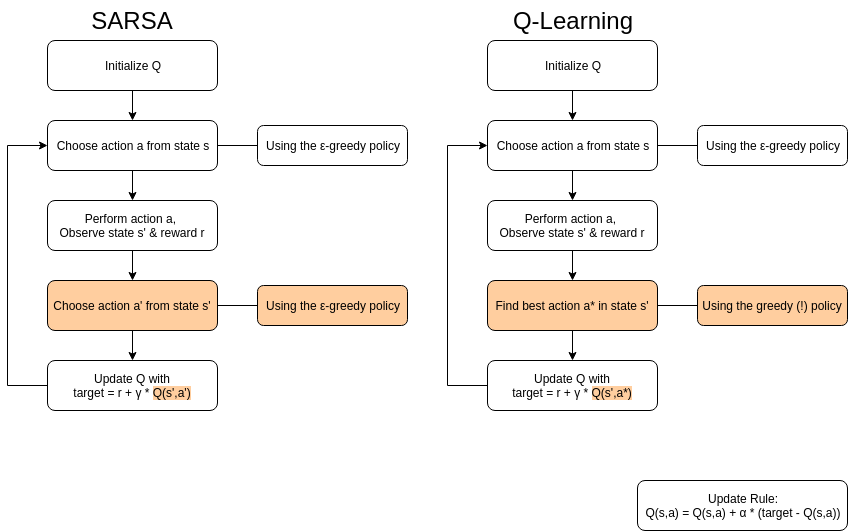
\includegraphics[width=1\linewidth]{img/SARSA_QL.png}
    \caption{Comparison of the Q-Learning and SARSA algorithms}
    \label{fig:ql_sarsa}
\end{figure}

In Q-learning, the agent follows the $\epsilon$-greedy policy in which we can vary the degree of exploration by adjusting $\epsilon$, the probability of taking a random action as opposed to the best action according to Q. This parameter allows for the exploration rate to start off with a high value such as 1, which causes the agent to choose only random actions, and then slowly decay over time to allow the agent to exploit its knowledge about the environment. At the same, Q is updated in a way that optimizes the greedy policy (see figure \ref{fig:ql_sarsa}). This is an off-policy algorithm.

In contrast, SARSA optimizes the same $\epsilon$-greedy policy that it is following. This makes it an on-policy algorithm and should see an increase in learning stability due to one less element of the deadly triad present in the system. Because SARSA updates Q in a way that takes into account the random actions the agent sometimes takes it is expected to find a safer, but less optimal policy \citep{sutton_barto_2018} and report a higher average performance during learning.

% make sure to explain what Q is in the RL section. maybe also what e-greedy looks like?



\subsubsection{Dueling Networks}\label{sec:dueling}
One limitation of the Q-Network approach is that it is not able to estimate the value of a state and the action separately \citep{wang2015dueling}. This ability can be very useful, since often in states an action has no relevant consequence. The Dueling Network Architecture achieves this by having two streams each predicting different things, instead of one stream predicting both. It is implemented by configuring two hidden layers in parallel, replacing the single hidden layer that is standard in the Q-Network. One of these two layers will estimate the state value, while the other layer will estimate the action advantages for each possible action. The two are merged together with the following formula:
$$ Q = value + (advantage - mean(advantage))$$
It automatically prevents the layer for the state value from estimating anything related to the action advantages, since the sum of these advantages is kept at zero. This formula results in the Q-values which can be used no different from the single stream Q-values. All learning techniques and code can be recycled. This modification is expected to boost the maximum performance, but especially the speed of learning.



\subsubsection{Demonstration Data}\label{sec:demo_data}
Because the reward function defined in section \ref{sec:reward_function} provides only sparse and delayed rewards, the agent might require additional guidance to learn to contain the fire in a reasonable training time. To point it in the right direction, we can fill the memory buffer with demonstration data before learning as mentioned in section \ref{sec:exp_replay}. The agent can then use these memories during the learning process to "see" a possible way to reach the sparse reward.

The demonstration data only needs to show the agent how it might be able to collect the containment reward, to this effect we developed a simple algorithm that moves the agent around the fire in a clockwise direction by choosing randomly from one of two possible actions depending on the position of the agent relative to the fire (shown schematically in figure \ref{fig:demodata}). 

The environment is reset upon containment (as defined in the algorithm \ref{alg:containment}), and if the agent would make a move that would lead to its death, it chooses the other possible action. Only memories leading to successful containments are kept. This results in an average of 35 demonstration data memories per containment of the fire, and the number of successful containments required can be specified.

\begin{figure}[h]
    \centering
    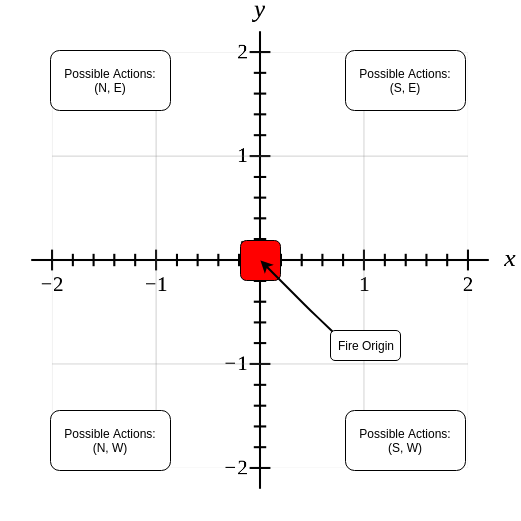
\includegraphics[width=1\linewidth]{img/Demo-data_Baseline.png}
    \caption{Possible actions to take, based on the agents position relative to the fire}
    \label{fig:demodata}
\end{figure}

% find and reference the paper introducing the demo data approach



\subsection{The Experimental Setup}\label{sec:experiment}

\subsubsection{Baseline Algorithm}\label{sec:baseline}
To be able to reliably compare the performance of the different algorithms, we need a stable baseline. We build on the ideas discussed in section \ref{sec:demo_data} to define the algorithm shown in \ref{alg:baseline}. This algorithm is identical to the demonstration data generation except that it continues until the fire has burnt out, and does not stop as soon as the fire is contained.

\begin{algorithm}
  \caption{Baseline algorithm to contain the fire}
  \label{alg:baseline}
  \begin{algorithmic}[1]
    \Procedure{RunBaseline}{}
    \State {totalreward = 0}
    \While {\textbf{not} done}
    \State {action = random(possible actions)}
    \If {action is dangerous}
    \State {action = other possible action}
    \EndIf
    \State {reward, done = execute(action)}
    \State {totalreward = totalreward + reward}
    \EndWhile
    \State \Return {totalreward}
    \EndProcedure
  \end{algorithmic}
\end{algorithm}

\subsubsection{Collection of Results}\label{sec:datacollection}
We investigate the performance of both Q-Learning and SARSA, both with and without the dueling network modification for a total of 4 different algorithms.

Each algorithm and parameter combination was run 10 times for 10,000 episodes per run. We compared the baseline performance to 2 map sizes (10x10, 14x14), 3 different amounts of demonstration data (0, 3,500, 35,000) and 4 algorithms for a total of 240 runs (260 including the baseline). Because each run took on average 4.5 hours, they were run on the Peregrine computing cluster provided by the University of Groningen.
